    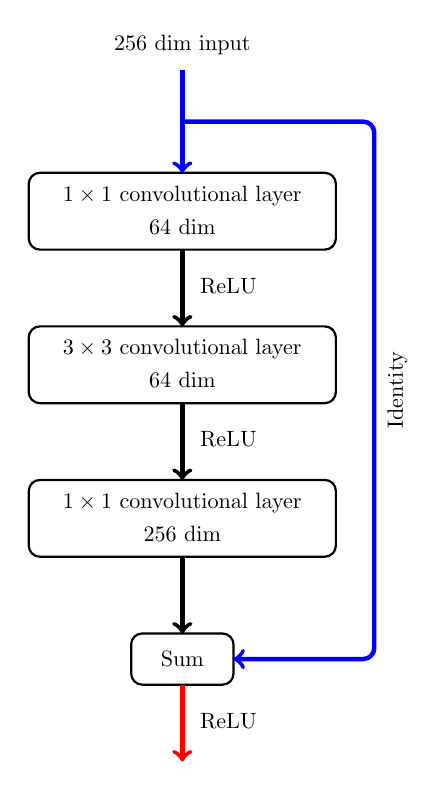
\begin{tikzpicture}[scale=0.65,every node/.style={scale=0.8}]

    \draw[black,thick,rounded corners] (0.5,0.0) rectangle (2.5,1.0);
    \node at (1.5,0.5) {Sum};

    \draw[black,thick,rounded corners] (-1.5,2.5) rectangle (4.5,4.0);
    \node at (1.5,3.55) {$1\times 1$ convolutional layer};
    \node at (1.5,2.95) {256 dim};

    \draw[black,thick,rounded corners] (-1.5,5.5) rectangle (4.5,7.0);
    \node at (1.5,6.55) {$3\times 3$ convolutional layer};
    \node at (1.5,5.95) {64 dim};

    \draw[black,thick,rounded corners] (-1.5,8.5) rectangle (4.5,10.0);
    \node at (1.5,9.55) {$1\times 1$ convolutional layer};
    \node at (1.5,8.95) {64 dim};

    \node at (1.5,12.5) {256 dim input};

    \draw[red,ultra thick,->] (1.5,0) -- (1.5,-1.5);
    \draw[black,ultra thick,->] (1.5,2.5) -- (1.5,1);
    \draw[black,ultra thick,->] (1.5,5.5) -- (1.5,4);
    \draw[black,ultra thick,->] (1.5,8.5) -- (1.5,7);
    \draw[blue,ultra thick,->] (1.5,12) -- (1.5,10);

    \node at (2.4,-0.7) {ReLU};
    \node at (2.4,4.8) {ReLU};
    \node at (2.4,7.8) {ReLU};

    \draw[blue,ultra thick,rounded corners,->] (1.5,11.0) -- (5.25,11.0) -- (5.25,0.5) -- (2.5,0.5);
    \node[rotate=90] at (5.7,5.75) {Identity};

%    \draw[black,ultra thick,rounded corners,->] (2.5,1) -- (2.5,2.5) -- (4,2.5);
%    \draw[black,ultra thick,rounded corners,->] (2.5,0) -- (2.5,-1.5) -- (4,-1.5);
%    \draw[red,ultra thick,dotted,->] (5.5,4.5) -- (5.5,3);
%    \draw[red,ultra thick,dotted,->] (5.5,-3.5) -- (5.5,-2);
%    \draw[black,ultra thick,rounded corners,->] (7,2.5) -- (9.75,2.5) -- (9.75,1);
%    \draw[black,ultra thick,rounded corners,->] (7,-1.5) -- (14.25,-1.5) -- (14.25,0);
%    \draw[black,ultra thick,->] (11.5,0.5) -- (12.5,0.5);
%    \draw[black,ultra thick,->] (16,0.5) -- (17,0.5);
     
    \end{tikzpicture}
